% ============================================================
% Analisi Matematica II -- Lezione 6: Topologia in R^n
% Fonti: appunti manoscritti (8 pagine) + registrazione audio
% (Analisi II - Lezione 6.m4a, 1:37:40)
% Da includere con \input; figure generate da figure.py
% ============================================================

% [0:00:13]
\section{Topologia in $\mathbb{R}^n$}

\paragraph{Perché serve.} Finora abbiamo studiato funzioni di una variabile
\[
  f\colon x\in[a,b]\longmapsto f(x)\in\mathbb{R},
\]
il cui grafico vive in $\mathbb{R}^2$. Ora vogliamo studiare funzioni di più variabili, a partire da due:
\[
  f(x,y)=z ,
\]
il cui grafico vive quindi in $\mathbb{R}^3$ (figura~\ref{fig:01}).
% [0:01:14]
La motivazione, per un fisico, è immediata: se una forza dipende dalla posizione di un corpo che si muove nel piano o nello spazio, la posizione è un vettore, e la forza deve dipendere da un vettore, non da un solo numero reale.

\begin{figure}[htbp]\centering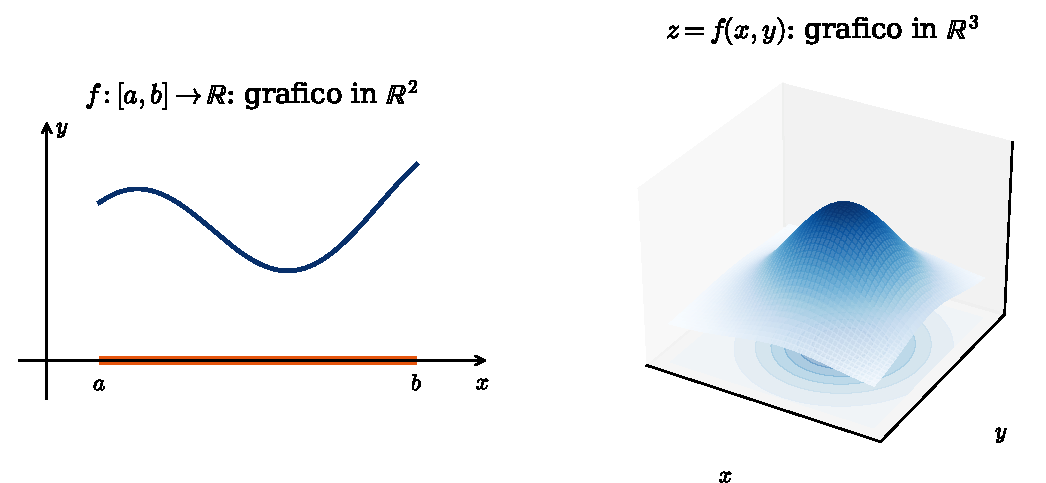
\includegraphics[width=0.85\linewidth]{figure/fig_01}\caption{Da una a due variabili: il grafico di $f\colon[a,b]\to\mathbb{R}$ sta in $\mathbb{R}^2$, quello di $z=f(x,y)$ in $\mathbb{R}^3$ (andamento qualitativo).}\label{fig:01}\end{figure}

% [0:03:45]
\paragraph{Osservazione.} Per le funzioni di più variabili \textbf{non esiste la monotonia}: tra vettori non c'è una relazione d'ordine. Tutti i teoremi sulle funzioni monotone di Analisi~I spariscono.

Per definire il limite di una funzione di più variabili servono, come in Analisi~I, un concetto di \emph{distanza}, di \emph{intorno}, di \emph{punto di accumulazione}, di \emph{aperto} e di \emph{chiuso}: è la topologia. Questa lezione è fondamentale anche per gli esercizi successivi (disegno dei domini, insiemi su cui integrare).
% [0:05:14]
Lavoreremo in $\mathbb{R}^2$ per poter fare i disegni, ma tutte le definizioni valgono in $\mathbb{R}^n$. C'è una sola cosa che si può fare in $\mathbb{R}^2$ e non in $\mathbb{R}^n$: definire \emph{l'}angolo tra due vettori (si veda il paragrafo sul prodotto scalare).

% [0:06:19]
\subsection{$\mathbb{R}^2$ come spazio vettoriale}

Sia
\[
  \mathbb{R}^2=\mathbb{R}\times\mathbb{R},
  \qquad\qquad
  \mathbb{R}^n=\underbrace{\mathbb{R}\times\dots\times\mathbb{R}}_{n\ \text{volte}} .
\]
Geometricamente $\mathbb{R}^2$ si rappresenta con il piano cartesiano (e $\mathbb{R}^3$ con tre assi). Su $\mathbb{R}^2$ (in generale su $\mathbb{R}^n$) si definiscono le seguenti operazioni.

\paragraph{Somma ($\oplus$).} Se $v_1=(x_1,y_1)$ e $v_2=(x_2,y_2)$ sono in $\mathbb{R}^2$,
\[
  v_1+v_2=(x_1+x_2,\;y_1+y_2).
\]
% [0:09:01]
È la stessa somma che si faceva con i numeri complessi, costruiti proprio su $\mathbb{R}^2$.

\paragraph{Prodotto per uno scalare ($\odot$).} Se $\alpha\in\mathbb{R}$ e $v=(x,y)\in\mathbb{R}^2$,
\[
  \alpha v=(\alpha x,\;\alpha y)\in\mathbb{R}^2 .
\]
Con queste operazioni $(\mathbb{R}^2,+,\cdot)$ è uno spazio vettoriale su $\mathbb{R}$; lo stesso vale per $\mathbb{R}^n$, operando componente per componente.

% [0:10:03]
\paragraph{Osservazione.} Il prodotto per uno scalare è un'operazione \emph{esterna}: combina uno scalare $\alpha\in\mathbb{R}$ con un elemento di $\mathbb{R}^2$, mentre un'operazione in senso stretto agisce tra elementi dello stesso insieme. Per questo alla lavagna i simboli $\oplus$, $\odot$ sono cerchiati: si sta \emph{definendo} l'operazione.

% [0:11:29]
\paragraph{Notazioni della docente.} Gli scalari si indicano sempre con lettere greche ($\alpha,\beta,\dots$); sui vettori non si mettono frecce o trattini: in caso di ambiguità si scrivono le componenti.

% [0:12:33]
\paragraph{Osservazione.} Poiché in uno spazio vettoriale esiste l'opposto ($-v_2$ ha le componenti di $v_2$ cambiate di segno), si definisce la differenza
\[
  v_1-v_2=v_1+(-v_2).
\]

% [0:12:33]
\subsection{Norma (modulo)}

\paragraph{Definizione.} Sia $v=(x,y)\in\mathbb{R}^2$. Si chiama \emph{norma} (o modulo) di $v$ la quantità
\[
  \|v\|=\sqrt{x^2+y^2}.
\]
In $\mathbb{R}^n$, con $v=(x_1,\dots,x_n)$:
\[
  \|v\|=\sqrt{x_1^2+\dots+x_n^2}.
\]

% [0:13:57]
Geometricamente è il teorema di Pitagora (figura~\ref{fig:02}). Per la docente $v$ è un \emph{punto} del piano (una coppia), non necessariamente la freccia che lo congiunge all'origine.

\begin{figure}[htbp]\centering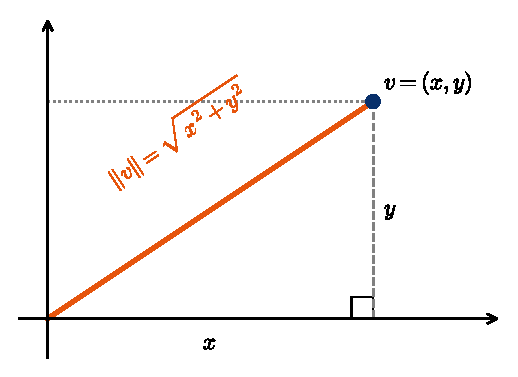
\includegraphics[width=0.5\linewidth]{figure/fig_02}\caption{La norma di $v=(x,y)$ è la lunghezza dell'ipotenusa: $\|v\|=\sqrt{x^2+y^2}$.}\label{fig:02}\end{figure}

% [0:15:21]
\paragraph{Osservazione (notazione).} Per $n=1$ si ottiene $\sqrt{x_1^2}=|x_1|$, cioè il valore assoluto. Per questo la docente indica la norma con \emph{una sola} sbarra, $|v|$, in tutte le dimensioni; la doppia sbarra $\|\cdot\|$, usata in questa dispensa, è l'altra notazione comune. La norma serve a calcolare le distanze, come il valore assoluto in Analisi~I.

% [0:16:50]
\paragraph{Proprietà della norma.}
\begin{enumerate}
  \item $\|v\|\geq 0$ per ogni $v\in\mathbb{R}^2$, e
  \[
    \|v\|=0 \iff v=0 \quad(\text{il vettore nullo});
  \]
  \item omogeneità:
  \[
    \|\alpha v\|=|\alpha|\,\|v\| \qquad \forall\,\alpha\in\mathbb{R},\ \forall\,v\in\mathbb{R}^2;
  \]
  % [0:18:12]
  (a sinistra c'è una norma in $\mathbb{R}^2$, a destra il valore assoluto in $\mathbb{R}$ di $\alpha$ moltiplicato per la norma di $v$);
  \item disuguaglianza triangolare:
  \[
    \|v_1+v_2\|\leq\|v_1\|+\|v_2\| \qquad \forall\,v_1,v_2\in\mathbb{R}^2 .
  \]
\end{enumerate}
Tutto vale anche in $\mathbb{R}^n$.

\paragraph{Definizione (norma astratta).} Se una funzione $f=\|\cdot\|$ definita su $\mathbb{R}^2$ (o, più in generale, su uno spazio vettoriale) soddisfa le tre proprietà precedenti, si chiama \emph{norma}.
% [0:19:24]
Il modo più corretto per il matematico è proprio questo: definire norma una qualunque funzione con queste proprietà, e poi verificare che $\sqrt{x^2+y^2}$ lo è.

% [0:19:24]
\paragraph{Dimostrazione geometrica della disuguaglianza triangolare.} In $\mathbb{R}^n$ la dimostrazione è identica a quella fatta in $\mathbb{R}$; in $\mathbb{R}^2$ c'è un'interpretazione geometrica che spiega il nome.
% [0:20:37]
La somma $v_1+v_2$ si costruisce con la regola del parallelogramma (figura~\ref{fig:03}). Il triangolo $T$ di vertici $0$, $v_1$, $v_1+v_2$ ha lati di lunghezza $\|v_1\|$, $\|v_2\|$ e $\|v_1+v_2\|$; poiché in un triangolo ogni lato è minore della somma degli altri due, si ha $\|v_1+v_2\|\leq\|v_1\|+\|v_2\|$.

\begin{figure}[htbp]\centering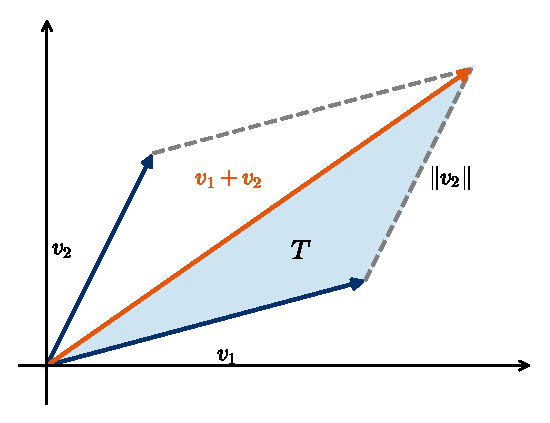
\includegraphics[width=0.55\linewidth]{figure/fig_03}\caption{Disuguaglianza triangolare: i lati del triangolo $T$ misurano $\|v_1\|$, $\|v_2\|$, $\|v_1+v_2\|$.}\label{fig:03}\end{figure}

% [0:21:47]
\paragraph{Esempio (una norma su uno spazio di funzioni).} Un insieme su cui è definita una norma si chiama \emph{spazio normato}, e non deve essere per forza $\mathbb{R}^2$ o $\mathbb{R}^n$. Sia
\[
  C([a,b])=\{f\colon[a,b]\to\mathbb{R}\ \text{continue}\}.
\]
% [0:23:06]
Non è un insieme di punti, ma di funzioni; con la somma di funzioni e il prodotto per uno scalare ha una struttura di spazio vettoriale. Si può introdurre una norma? Sì:
\[
  \|f\|=\max_{[a,b]}|f| .
\]
La definizione è ben posta perché, per il teorema di Weierstrass, una funzione continua su $[a,b]$ ammette massimo.
% [0:24:17]
Nei testi si trova anche scritta $\|f\|_\infty$. È una norma: è $\geq 0$ e vale $0$ solo se $|f|$ è identicamente nulla; l'omogeneità è immediata; vale la disuguaglianza triangolare perché il massimo di $|f+g|$ è minore o uguale alla somma dei massimi di $|f|$ e $|g|$.
% [0:25:25]
Tutto ciò che si fa per i vettori si generalizza quindi a qualunque spazio vettoriale dotato di norma: sarà il punto di partenza del corso di Metodi, dove si lavora con spazi di funzioni.

% [0:25:25]
\subsection{Distanza}

\paragraph{Definizione.} Siano $v_1=(x_1,y_1)$ e $v_2=(x_2,y_2)$ in $\mathbb{R}^2$. Si chiama \emph{distanza} tra $v_1$ e $v_2$ la quantità
\[
  d(v_1,v_2)=\|v_1-v_2\|=\sqrt{(x_1-x_2)^2+(y_1-y_2)^2}.
\]
% [0:26:48]
È la distanza tra due punti che si calcolava a scuola.
% [0:28:10]
Come in Analisi~I, la norma evita di dover discutere quale dei due punti è ``più grande'': in $\mathbb{R}$ la distanza tra $x$ e $y$ è $|x-y|$, senza distinguere i casi $x-y$ e $y-x$. La distanza eredita tutte le proprietà della norma: è sempre $\geq 0$ e si annulla solo se i due punti coincidono.

\paragraph{Attenzione.} In $\mathbb{R}^2$ (e in generale in $\mathbb{R}^n$) \textbf{non c'è una relazione d'ordine}: non si possono confrontare i vettori, non esiste il ``$\leq$''.

% [0:29:35]
\subsection{Prodotto scalare}

\paragraph{Definizione.} Siano $v_1=(x_1,y_1)$ e $v_2=(x_2,y_2)$ in $\mathbb{R}^2$. Si chiama \emph{prodotto scalare} tra $v_1$ e $v_2$
\[
  \langle v_1,v_2\rangle := x_1x_2+y_1y_2\in\mathbb{R}.
\]
In $\mathbb{R}^n$ si aggiungono semplicemente gli altri prodotti componente per componente.
% [0:30:49]
La docente usa sempre le parentesi angolari perché le altre notazioni sono ambigue: le parentesi tonde sembrano un intervallo, il solo punto sembra un prodotto tra numeri.
% [0:35:19]
Attenzione: il prodotto scalare prende in input due vettori e restituisce un \emph{numero reale}.

% [0:32:17]
\paragraph{Osservazione.} In $\mathbb{R}^2$ è noto anche che
\[
  \langle v_1,v_2\rangle=\|v_1\|\,\|v_2\|\cos\theta ,
\]
dove $\theta$ è l'angolo tra i due vettori, preso in $[0,\pi]$ (figura~\ref{fig:04}). Questa non è la definizione, ma un teorema.
% [0:34:01]
In dimensione maggiore di $2$ non esiste ``l'''angolo tra due vettori: servono più angoli (in $\mathbb{R}^n$ ne servono $n-1$), come nelle coordinate polari. In $\mathbb{R}^2$ un punto si individua con modulo e un angolo; in $\mathbb{R}^3$, ad esempio sulla sfera, servono due angoli, uno dei quali misura la rotazione attorno all'asse $z$.
% [0:36:32]
(Prendere il piano individuato dai due vettori significa di fatto tornare in $\mathbb{R}^2$.) Per questo la definizione per componenti è l'unica che vale in tutte le dimensioni ed è quella che si usa.

\begin{figure}[htbp]\centering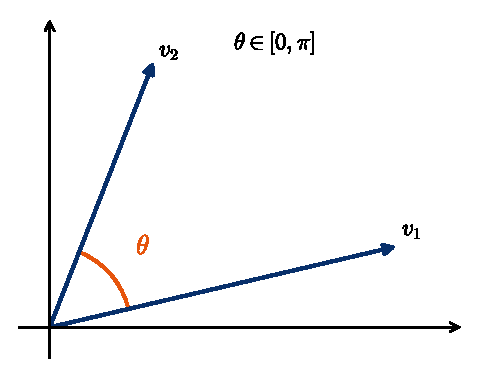
\includegraphics[width=0.5\linewidth]{figure/fig_04}\caption{L'angolo $\theta\in[0,\pi]$ tra due vettori di $\mathbb{R}^2$.}\label{fig:04}\end{figure}

% [0:37:49]
\paragraph{Proprietà del prodotto scalare.} Per ogni $v_1,v_2,v_3\in\mathbb{R}^2$ (in generale $\mathbb{R}^n$) e per ogni $\alpha\in\mathbb{R}$:
\begin{enumerate}
  \item simmetria (commutatività):
  \[
    \langle v_1,v_2\rangle=\langle v_2,v_1\rangle;
  \]
  \item linearità rispetto alla somma:
  \[
    \langle v_1+v_2,v_3\rangle=\langle v_1,v_3\rangle+\langle v_2,v_3\rangle;
  \]
  \item linearità rispetto al prodotto per uno scalare:
  \[
    \alpha\langle v_1,v_2\rangle=\langle\alpha v_1,v_2\rangle=\langle v_1,\alpha v_2\rangle;
  \]
  (per la simmetria, 2 e 3 valgono in entrambi gli argomenti: il prodotto scalare è bilineare)
  % [0:39:16]
  \item il prodotto scalare di un vettore per se stesso dà la norma al quadrato:
  \[
    \langle v_1,v_1\rangle=\|v_1\|^2;
  \]
  \item disuguaglianza di Cauchy--Schwarz:
  \[
    |\langle v_1,v_2\rangle|\leq\|v_1\|\,\|v_2\| .
  \]
\end{enumerate}
La disuguaglianza di Cauchy--Schwarz è fondamentale: servirà per le derivate, e senza di essa non si potrebbe definire l'angolo (è lei a garantire che $\langle v_1,v_2\rangle/(\|v_1\|\,\|v_2\|)$ stia in $[-1,1]$ e quindi sia un coseno).

% [0:40:31]
\subsection{Intorni sferici}

Da qui in poi $\mathbb{R}^2$ non ha più nulla di speciale: tutto vale in $\mathbb{R}^n$.

\paragraph{Definizione.} Sia $v_0=(x_0,y_0)\in\mathbb{R}^2$ e sia $\delta>0$. Si chiama \emph{intorno sferico} di $v_0$ di raggio $\delta$ l'insieme
\[
  I_\delta(v_0)=B_\delta(v_0)=\bigl\{v=(x,y)\in\mathbb{R}^2 : \|v-v_0\|<\delta\bigr\}.
\]
% [0:41:52]
Per $n=1$ la stessa definizione restituisce l'intervallo aperto $(x_0-\delta,\,x_0+\delta)$.
% [0:43:09]
Sostituendo la formula della distanza:
\[
  I_\delta(v_0)=\Bigl\{(x,y)\in\mathbb{R}^2 : \sqrt{(x-x_0)^2+(y-y_0)^2}<\delta\Bigr\},
\]
ovvero
\[
  (x-x_0)^2+(y-y_0)^2<\delta^2 .
\]
Con l'uguale questa è l'equazione di una circonferenza di centro $(x_0,y_0)$ e raggio $\delta$; con il minore stretto è il cerchio (disco) \emph{senza} la circonferenza di bordo (figura~\ref{fig:05}, a sinistra). Da qui il nome ``sferico'' e la notazione $B$ (in inglese \emph{ball}).

% [0:44:11]
\paragraph{Osservazione.} In Analisi~I, per ``stare vicino'' a $x_0$ si prendevano intervalli aperti centrati in $x_0$. In Analisi~II stare vicino a un punto significa ``prendere la mira'' con un mirino circolare: il disco raccoglie tutte le direzioni attorno al punto, a $360^\circ$. In dimensione più alta gli intorni sono palle.
% [0:45:13]
Le nozioni di punto interno, aperto, chiuso, ecc.\ dipendono \emph{solo} dalla definizione di intorno: le definizioni di Analisi~I si possono ricopiare parola per parola. Cambia solo l'intorno, che eredita le proprietà della distanza dello spazio in cui si lavora.
% [0:46:34]
Questo vale in ogni spazio normato: ad esempio si può parlare di intorno di una funzione in $C([a,b])$.

% [0:47:52]
\paragraph{Esempio (un'altra norma).} Quella euclidea non è l'unica norma possibile su $\mathbb{R}^2$. Per $v=(x,y)$ si ponga
\[
  \|v\|:=\max\{|x|,|y|\}.
\]
Anche questa verifica le tre proprietà della norma. Chi sono gli intorni ``sferici'' per questa norma? Centrando in $0$,
% [0:49:14]
\[
  \|v\|<\delta \iff |x|<\delta\ \ \text{e}\ \ |y|<\delta ,
\]
cioè sono \textbf{quadrati} in $\mathbb{R}^2$ (e \textbf{cubi} in $\mathbb{R}^3$). Ad esempio l'intorno $\|v\|<1$ è il quadrato aperto $(-1,1)\times(-1,1)$ (figura~\ref{fig:05}, a destra).

\begin{figure}[htbp]\centering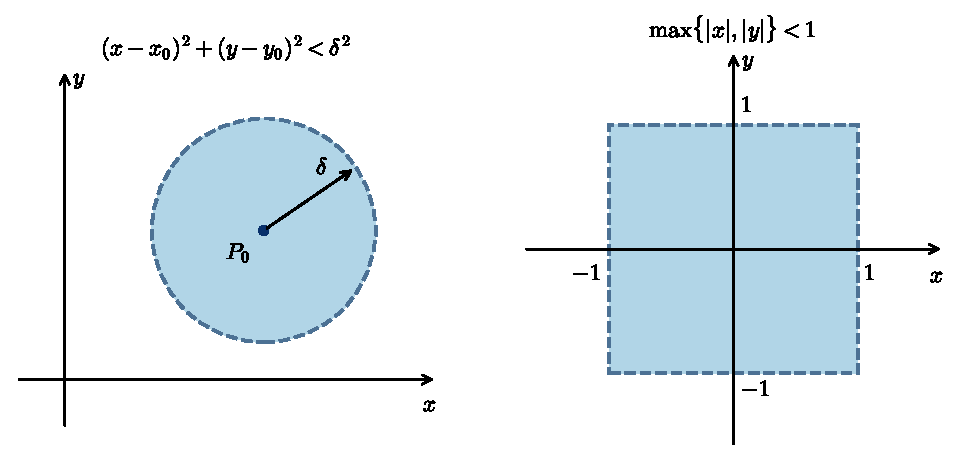
\includegraphics[width=0.85\linewidth]{figure/fig_05}\caption{Intorni sferici: il disco aperto della norma euclidea (sinistra) e il quadrato aperto della norma del massimo (destra). Bordo tratteggiato: non appartiene all'insieme.}\label{fig:05}\end{figure}

% [0:50:22]
\subsection{Punti interni, esterni, di frontiera, isolati}

\paragraph{Definizione.} Sia $A\subseteq\mathbb{R}^2$ e $v_0=(x_0,y_0)\in A$. Il punto $(x_0,y_0)$ si dice \emph{interno} ad $A$ se
\[
  \exists\, I_\delta(x_0,y_0)\subset A ,
\]
cioè se esiste tutta una ``palletta'' centrata nel punto e contenuta in $A$.

% [0:51:45]
\paragraph{Definizione.} Un punto $(x_0,y_0)\in\mathbb{R}^2$ si dice \emph{esterno} ad $A$ se
\[
  \exists\, I_\delta(x_0,y_0) : I_\delta(x_0,y_0)\cap A=\emptyset ,
\]
cioè se ha un intorno contenuto nel complementare di $A$.

% [0:53:10]
\paragraph{Definizione.} Un punto $(x_0,y_0)\in\mathbb{R}^2$ si dice \emph{di frontiera} per $A$ se non è né interno né esterno, ovvero se
\[
  \forall\, I_\delta(x_0,y_0):\quad I_\delta(x_0,y_0)\cap A\neq\emptyset
  \quad\text{e}\quad I_\delta(x_0,y_0)\setminus A\neq\emptyset .
\]
Ogni palletta attorno a un punto di frontiera ``becca'' sia punti di $A$ sia punti fuori da $A$ (figura~\ref{fig:06}).

\begin{figure}[htbp]\centering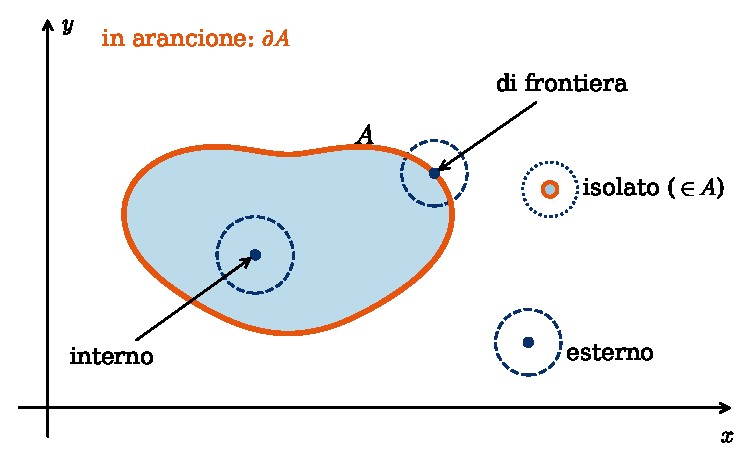
\includegraphics[width=0.7\linewidth]{figure/fig_06}\caption{Punto interno, di frontiera, esterno e isolato per un insieme $A$. In arancione la frontiera $\partial A$.}\label{fig:06}\end{figure}

% [0:54:28]
In $\mathbb{R}$ la frontiera era data dagli estremi: gli insiemi tipici sono intervalli e la loro frontiera sono i due ``tappi''. In $\mathbb{R}^2$ la frontiera è un oggetto nuovo, che si disegna: una \emph{curva} (figura~\ref{fig:07}). Le curve saranno l'argomento delle prossime lezioni. Le nozioni di punto interno ed esterno sono così intuitive che basta guardare il disegno: l'analisi diventa visiva.

\begin{figure}[htbp]\centering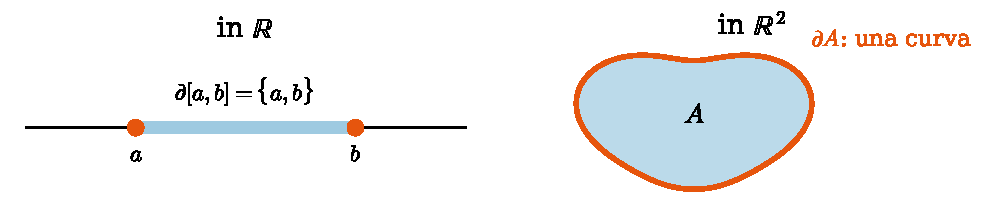
\includegraphics[width=0.8\linewidth]{figure/fig_07}\caption{La frontiera di un intervallo di $\mathbb{R}$ è fatta dai due estremi; quella di un insieme di $\mathbb{R}^2$ è una curva.}\label{fig:07}\end{figure}

% [0:55:31]
\paragraph{Definizione.} L'insieme dei punti di frontiera di $A$ si indica con $\partial A$ e si chiama \emph{frontiera} di $A$: è il ``contorno'' dell'insieme.

% [0:56:54]
\paragraph{Definizione.} Un punto $(x_0,y_0)\in\mathbb{R}^2$ si dice \emph{isolato} per $A$ se
\[
  \exists\, I_\delta(x_0,y_0) : I_\delta(x_0,y_0)\cap A=\{(x_0,y_0)\}.
\]
Ad esempio, se $A$ è l'insieme disegnato in figura~\ref{fig:06} unito a un punto ``staccato'', quel punto è isolato. I punti interni non sono mai isolati.
% [0:59:36]
Capitava già in Analisi~I (un intervallo unito a un punto). In un punto isolato non ha senso studiare la continuità o il limite, perché non ci si può avvicinare: per questo serve la nozione di punto di accumulazione.

% [0:56:54]
\subsection{Insiemi aperti e chiusi}

\paragraph{Definizione.} Un insieme $A\subseteq\mathbb{R}^2$, $A\neq\emptyset$, si dice \emph{aperto} se tutti i suoi punti sono interni.

\paragraph{Definizione.} Un insieme $C\subseteq\mathbb{R}^2$ si dice \emph{chiuso} se il suo complementare è aperto.

% [0:58:16]
Nei disegni: dove il bordo è tratteggiato, il bordo \emph{non} appartiene all'insieme; dove è continuo, appartiene. Come un intervallo aperto non contiene i ``tappi'', un aperto di $\mathbb{R}^2$ non deve contenere nessun punto del suo contorno (altrimenti quei punti sarebbero di frontiera, non interni). Un chiuso, invece, deve contenere la sua frontiera.

% [0:59:36]
\paragraph{Esempi.} Si veda la figura~\ref{fig:08}:
\begin{itemize}
  \item un insieme che contiene solo una parte del suo bordo non è aperto (contiene punti di frontiera) e non è nemmeno chiuso (non contiene tutta la frontiera);
  % [1:00:29]
  \item il semipiano che sta sopra una retta, retta compresa, è chiuso, ma non limitato; se la retta è tratteggiata diventa un aperto illimitato;
  \item un disco con il bordo continuo è chiuso;
  \item un insieme con il bordo tratteggiato è aperto.
\end{itemize}

\begin{figure}[htbp]\centering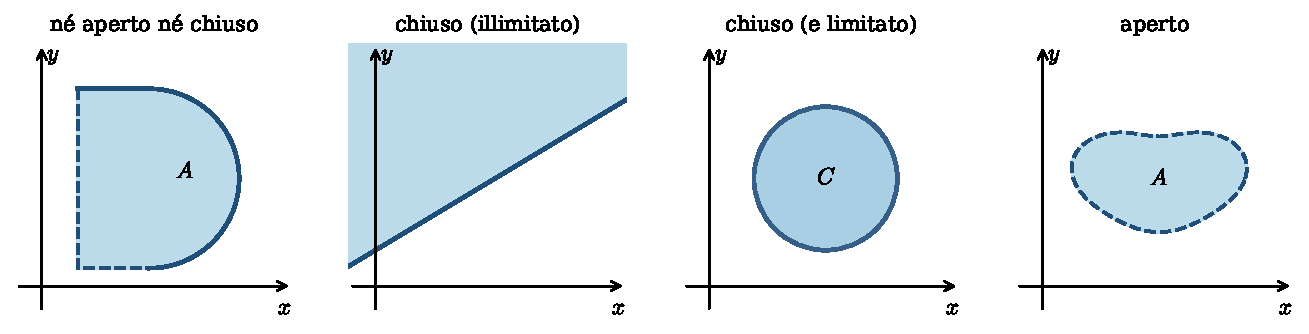
\includegraphics[width=\linewidth]{figure/fig_08}\caption{Da sinistra: insieme né aperto né chiuso; semipiano chiuso illimitato; disco chiuso; insieme aperto.}\label{fig:08}\end{figure}

% [1:00:29]
\subsection{Punti di accumulazione, insiemi limitati e compatti}

\paragraph{Definizione.} Sia $A\subseteq\mathbb{R}^2$ con $A\neq\emptyset$. Il punto $(x_0,y_0)$ si dice \emph{di accumulazione} per $A$ se
\[
  \forall\, I_\delta(x_0,y_0):\quad \bigl(I_\delta(x_0,y_0)\cap A\bigr)\setminus\{(x_0,y_0)\}\neq\emptyset .
\]
% [1:01:23]
Cioè ci si può avvicinare quanto si vuole a $(x_0,y_0)$ con punti di $A$ diversi da $(x_0,y_0)$.

Valgono le stesse caratterizzazioni di Analisi~I:
\[
  A\ \text{chiuso} \iff A\ \text{contiene tutti i suoi punti di accumulazione}
  \iff A\ \text{contiene la sua frontiera}.
\]

\paragraph{Definizione.} Un insieme $A\subseteq\mathbb{R}^2$, $A\neq\emptyset$, si dice \emph{limitato} se
\[
  \exists\, I_R(0) : A\subset I_R(0).
\]
% [1:02:38]
Al posto di $0$ si può mettere qualunque centro. Essere limitato significa poter chiudere l'insieme dentro una ``bolla'' (non per forza circoscritta: può essere anche più grande). Un semipiano non è limitato: per quanto grande si prenda il raggio, non lo si racchiude mai tutto.

\paragraph{Definizione.} Un insieme $K\subseteq\mathbb{R}^2$ si dice \emph{compatto} se è chiuso e limitato.

% [1:04:06]
\paragraph{Osservazione.} In realtà questa ``definizione'' è il contenuto del teorema di Heine--Borel, visto in Analisi~I in $\mathbb{R}$. La definizione vera di compatto in $\mathbb{R}^n$ richiederebbe le successioni di vettori e il loro limite (da ogni successione si deve poter estrarre una sottosuccessione convergente); poi si dimostrerebbe l'analogo di Heine--Borel. Per semplicità si assume direttamente ``compatto = chiuso e limitato''.
% [1:05:08]
Ad esempio: un disco chiuso è compatto; un disco aperto non lo è (non è chiuso); un semipiano chiuso non lo è (non è limitato).

% [1:05:08]
\subsection{Esercizio: disegnare regioni del piano}

Da qui si entra nel vivo delle due dimensioni. Come in Analisi~I si leggevano le proprietà di una funzione dal grafico, ora si disegnano regioni di $\mathbb{R}^2$ e se ne leggono le proprietà topologiche.

% [1:07:06]
\paragraph{Esercizio.} Disegnare la regione
\[
  E=\bigl\{(x,y)\in\mathbb{R}^2 : |y|<x,\ \ x^2+y^2\leq 3,\ \ x^2>y\bigr\}
\]
e stabilire se è aperta, chiusa, limitata, compatta; determinare la frontiera, i punti interni e i punti esterni.

% [1:08:06]
\paragraph{Definizione (parte interna e chiusura).} Sia $A\subseteq\mathbb{R}^2$.
\begin{itemize}
  \item La \emph{parte interna} di $A$, indicata con $\mathring{A}$, è il più grande aperto contenuto in $A$: in pratica $A$ privato della sua frontiera (nel disegno, il bordo diventa tutto tratteggiato).
  \item La \emph{chiusura} di $A$ è
  \[
    \overline{A}=A\cup\partial A ,
  \]
  che è un chiuso (nel disegno, il bordo diventa tutto continuo).
\end{itemize}

% [1:08:06]
\paragraph{Da dove viene $E$.} Una regione come $E$ nasce come dominio di una funzione di due variabili. Si consideri
\[
  f(x,y)=\frac{\log\bigl(x-|y|\bigr)+\sqrt{3-(x^2+y^2)}}{\sqrt[4]{x^2-y}} .
\]
% [1:10:58]
Non servono nuove funzioni elementari: si usano quelle di Analisi~I mettendoci dentro sia $x$ sia $y$, e il risultato è sempre un numero reale. Si cercano le coppie $(x,y)$ per cui ogni pezzo si può calcolare nel senso di Analisi~I:
\[
  \begin{cases}
    x-|y|>0 & \text{(argomento del logaritmo positivo)}\\[2pt]
    3-(x^2+y^2)\geq 0 & \text{(radice quadrata definita)}\\[2pt]
    x^2-y>0 & \text{(radice quarta definita e denominatore non nullo)}
  \end{cases}
\]
che è esattamente $E$.
% [1:09:30]
A differenza di Analisi~I, queste disequazioni in due variabili \emph{non} si risolvono (si saprebbe farlo solo per sistemi lineari): si \emph{disegnano}. Il disegno serve perché se il dominio ha buone proprietà, la funzione ha buone proprietà; e perché regioni come questa torneranno come domini negli esercizi d'esame e come insiemi di integrazione.

% [1:12:14]
\paragraph{Metodo.}
\begin{enumerate}
  \item Si disegnano tutti i \emph{casi di uguaglianza}: qui le rette $y=\pm x$, la parabola $y=x^2$ e la circonferenza $x^2+y^2=3$. Oltre ai grafici delle funzioni elementari possono comparire ``luoghi geometrici'' (circonferenze, ellissi\ldots).
  % [1:13:31]
  \item Si sceglie la parte giusta: per un \emph{grafico}, ``$>$'' significa sopra e ``$<$'' sotto; per un \emph{luogo geometrico} come una circonferenza, ``$<$'' significa dentro e ``$>$'' fuori.
  \item Se la disuguaglianza è stretta il bordo si tratteggia (non appartiene); se è larga si lascia continuo.
\end{enumerate}

% [1:14:38]
\paragraph{Svolgimento.} (Figura~\ref{fig:09}.)
\begin{itemize}
  \item $|y|<x$: il bordo $x=|y|$ è la ``V'' del valore assoluto ruotata (il ruolo di $x$ e $y$ è scambiato); si prende il settore a destra, compreso tra le rette $y=x$ e $y=-x$, con i bordi tratteggiati.
  % [1:16:03]
  \item $y<x^2$: si prendono i punti sotto la parabola $y=x^2$, con la parabola tratteggiata. Intersecando con il settore, per $0<x<1$ la parabola sta sotto la retta $y=x$ e taglia via la parte alta del settore.
  % [1:18:10]
  \item $x^2+y^2\leq 3$: disco di centro $(0,0)$ e raggio $\sqrt{3}$, bordo continuo.
\end{itemize}
Il risultato è una ``fetta di torta'' il cui arco di circonferenza è continuo, mentre i bordi rettilinei e parabolico sono tratteggiati.

\begin{figure}[htbp]\centering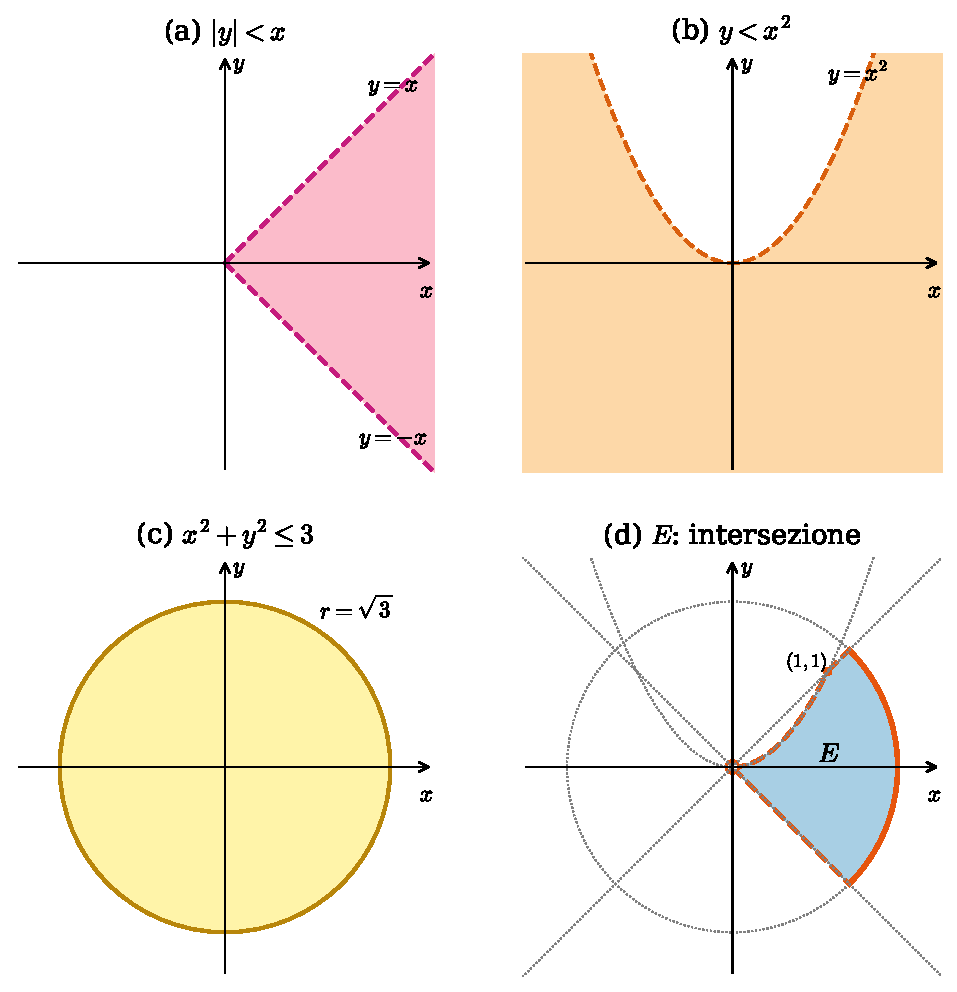
\includegraphics[width=0.5\linewidth]{figure/fig_09}\caption{Costruzione di $E=\{|y|<x,\ x^2+y^2\leq3,\ y<x^2\}$. In (d): bordo tratteggiato = non appartiene a $E$, continuo = appartiene; l'origine non appartiene a $E$.}\label{fig:09}\end{figure}

% [1:19:42]
\paragraph{Conclusione.} $E$ è \textbf{né aperto né chiuso} (contiene l'arco di circonferenza ma non gli altri pezzi di bordo) ed è \textbf{limitato} (quindi non compatto, perché non chiuso). La frontiera $\partial E$ è formata dall'arco di circonferenza, dal tratto di parabola e dai tratti delle rette $y=\pm x$.
% [1:20:23]
Per disegnare questi ``luoghi'' serve richiamare circonferenze, ellissi, ecc.: per questo le prossime lezioni saranno sulle curve.

% [1:21:17]
\subsection{Insiemi connessi}

\paragraph{Definizione.} Sia $A\subseteq\mathbb{R}^2$, $A\neq\emptyset$ e $A$ aperto. $A$ si dice \emph{connesso} se, ogni volta che esistono $A_1,A_2$ aperti tali che
\[
  A=A_1\cup A_2 \qquad\text{e}\qquad A_1\cap A_2=\emptyset ,
\]
allora deve essere $A_1=\emptyset$ e $A_2=A$ (o viceversa). In altre parole, $A$ non si può spezzare in due aperti disgiunti non vuoti.

% [1:22:34]
\paragraph{Osservazione.} La definizione è molto astratta, ma è l'unico modo rigoroso di dire ciò che si vede intuitivamente: un insieme è connesso se è sempre possibile ``collegare'' due suoi punti, cioè raggiungere l'uno dall'altro in qualche modo, non per forza in linea retta (``non si arriva a Roma in linea retta, ma si è comunque collegati''). Dire ``collegare'' senza specificare con cosa sarebbe impreciso; la definizione dice invece che l'insieme non è fatto di pezzi scollegati, cioè non è unione di parti disgiunte.
% [1:35:40]
Immagine: se si divide l'aula con un muro si ottengono due stanze isolate, due aperti disgiunti la cui unione è tutta l'aula; l'aula divisa è sconnessa.
% [1:36:49]
Analogamente, un foglio tagliato con le forbici fino ai bordi diventa unione di due pezzi scollegati, anche se li si tiene vicini: i due pezzi si chiamano \emph{componenti connesse}.

% [1:22:34]
\paragraph{Esempio.} La \emph{clessidra senza frontiera} (due triangoli aperti opposti al vertice, origine esclusa) è un aperto \textbf{non connesso}: i due triangoli sono due aperti disgiunti $A_1$, $A_2$ e non è possibile collegare un punto dell'uno con un punto dell'altro, perché l'origine non appartiene all'insieme (figura~\ref{fig:10}).

\begin{figure}[htbp]\centering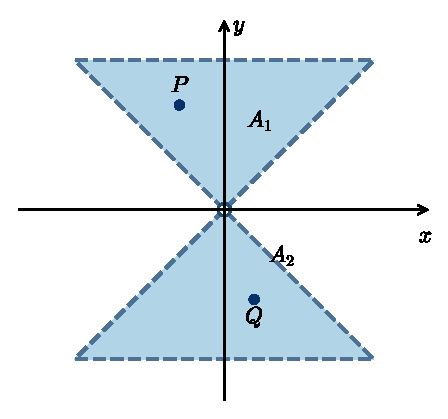
\includegraphics[width=0.45\linewidth]{figure/fig_10}\caption{Clessidra senza frontiera: aperto sconnesso, unione dei due aperti disgiunti $A_1$ e $A_2$.}\label{fig:10}\end{figure}

% [1:24:54]
\paragraph{Osservazione.} La definizione è data per insiemi aperti. Se $A\subseteq\mathbb{R}^2$, $A\neq\emptyset$, non è aperto, si dice che $A$ è connesso se lo è la sua parte interna $\mathring{A}$.

% [1:26:15]
\subsection{Insiemi convessi}

\paragraph{Definizione.} Sia $A\subseteq\mathbb{R}^2$, $A\neq\emptyset$ (non necessariamente aperto). $A$ si dice \emph{convesso} se per ogni coppia di punti $p,q\in A$ il segmento che li congiunge è contenuto in $A$.

% [1:27:34]
\paragraph{Esempi.} (Figura~\ref{fig:11}.) Un cerchio, un'ellisse, un segmento sono convessi. Un insieme a forma di ``C'' (o di ``S'') non è convesso: ci sono due punti il cui segmento esce dall'insieme. Una corona circolare (``la ciambella'') non è convessa, perché il segmento tra due punti opposti attraversa il buco; però è connessa, perché i due punti si possono comunque collegare girando attorno al buco.

\begin{figure}[htbp]\centering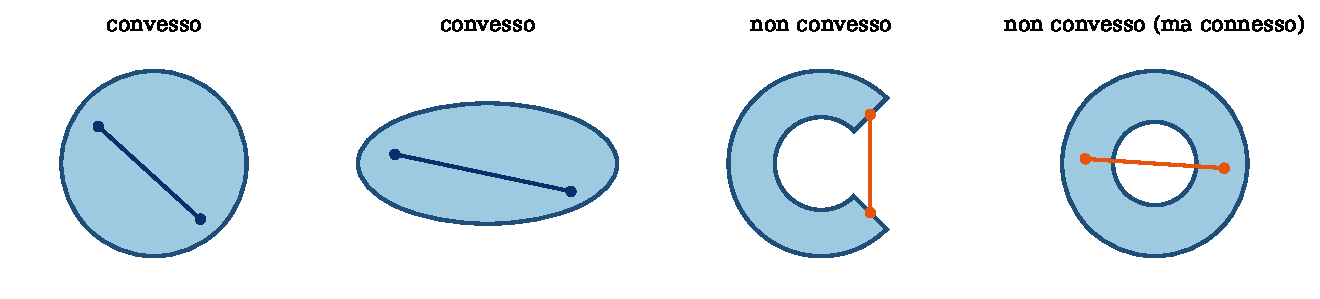
\includegraphics[width=\linewidth]{figure/fig_11}\caption{Insiemi convessi (disco, ellisse) e non convessi (insieme a forma di C, corona circolare): in arancione un segmento con estremi nell'insieme che ne esce.}\label{fig:11}\end{figure}

% [1:28:08]
\paragraph{Osservazione.} È ovvio che
\[
  \text{convesso} \implies \text{connesso},
\]
mentre la corona circolare mostra che non vale il viceversa: la convessità è più forte.

% [1:28:08]
\subsection{Insiemi stellati}

\paragraph{Definizione.} $A\subseteq\mathbb{R}^2$ si dice \emph{stellato rispetto a} $(x_0,y_0)$ se per ogni $p\in A$ il segmento che congiunge $p$ a $(x_0,y_0)$ è contenuto in $A$. Il punto $(x_0,y_0)$ si chiama \emph{centro della stella}.

% [1:29:40]
\paragraph{Esempio.} La \emph{clessidra chiusa} (due triangoli chiusi opposti al vertice) non è convessa: due punti presi uno in alto e uno in basso non sono collegati da un segmento contenuto nell'insieme. È però stellata rispetto al vertice comune: ogni punto si collega con un segmento al centro (figura~\ref{fig:12}, sinistra). Basta trovare \emph{un} centro: rispetto ad altri punti la stessa figura non è stellata.

% [1:30:52]
\paragraph{Osservazione.} Un convesso è stellato rispetto a \emph{qualunque} suo punto:
\[
  \text{convesso} \implies \text{stellato},
\]
mentre stellato non implica convesso (la clessidra chiusa).
% [1:29:40]
In Analisi~I nessuna di queste distinzioni aveva senso: in $\mathbb{R}$ gli insiemi di interesse erano intervalli, e un intervallo contiene sempre i segmenti tra i suoi punti, perché è esso stesso un segmento.

% [1:31:57]
\subsection{Connessione per poligonali}

\paragraph{Definizione.} Sia $A\subseteq\mathbb{R}^2$, $A\neq\emptyset$. $A$ si dice \emph{connesso per poligonali} se per ogni $p_1,p_2\in A$ esiste una spezzata (unione di segmenti) che li congiunge ed è contenuta in $A$.

% [1:31:57]
\paragraph{Osservazione.} Il legame con la connessione c'è, ma con una sottile differenza: la definizione di connessione vale per gli aperti, quella per poligonali no. Per gli \textbf{aperti}, connessione e connessione per poligonali coincidono. Per insiemi non aperti ci sono insiemi connessi per poligonali ma non connessi. (Nei testi le definizioni non sono sempre date esattamente così: alcuni danno tutto solo per gli aperti.)

% [1:33:16]
\paragraph{Esempio.} La clessidra chiusa è connessa per poligonali: due punti dei due triangoli si collegano con una spezzata di due segmenti passando per l'origine (figura~\ref{fig:12}, destra). Non è però connessa: per verificarlo si deve guardare la parte interna, che toglie i bordi e quindi anche l'origine, punto di raccordo; ciò che resta è la clessidra aperta della figura~\ref{fig:10}, che è sconnessa.

\begin{figure}[htbp]\centering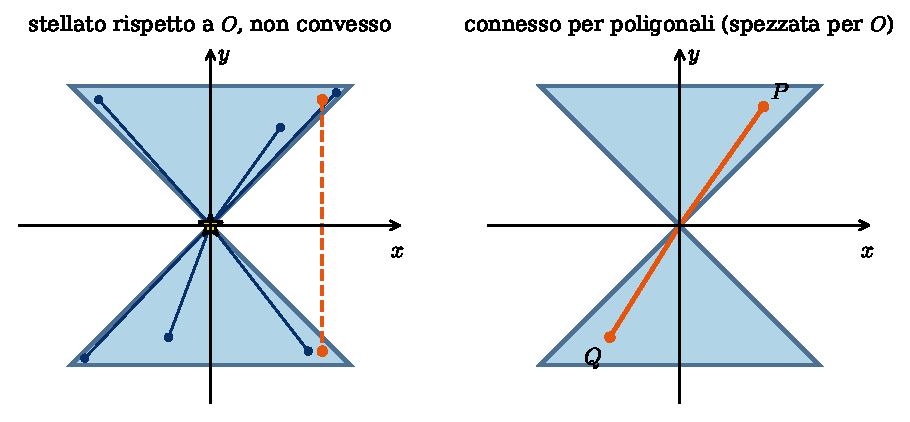
\includegraphics[width=0.85\linewidth]{figure/fig_12}\caption{Clessidra chiusa. Sinistra: stellata rispetto all'origine $O$ ma non convessa (il segmento arancione esce dall'insieme). Destra: connessa per poligonali tramite una spezzata che passa per $O$.}\label{fig:12}\end{figure}

% [1:36:49]
\paragraph{Perché servono queste nozioni.} Nel teorema degli zeri, se una funzione assume valori di segno opposto in due punti, per concludere che si annulla in mezzo serve che ciò che sta ``tra'' i due punti (ad esempio il segmento che li unisce) sia contenuto nell'insieme. Chi garantisce che sia così? Si pensi alla ciambella o all'insieme a forma di C. La forma del dominio diventa quindi fondamentale per ritrovare i risultati di Analisi~I.

% ============================================================
% DUBBI:
% - p. 1: "C'è solo una cosa che in R^n non si può fare ma in R^2 sì":
%   negli appunti non è esplicitata; dall'audio [0:34:01], [0:40:31]
%   è la nozione di angolo (unico) tra due vettori. Inserita così.
% - p. 1 [0:10:03]: la parte sulla formula di alpha*v dettata a voce
%   è confusa nella trascrizione; formula presa dagli appunti.
% - p. 2-3: la docente usa |v| (sbarra singola) per la norma, gli
%   appunti alternano ||v|| e |v|. Nella dispensa: ||v|| ovunque
%   (spiegato in un'osservazione).
% - p. 3: "La distanza è anch'essa norma" (appunti) è impreciso: la
%   distanza è una funzione di due punti che eredita le proprietà della
%   norma [0:28:10], non una norma. Riformulato.
% - p. 3: "forall v_1 - v_3" letto come "per ogni v_1, v_2, v_3" [0:40:31].
% - p. 4: il docente scrive il centro dell'intorno come P_0; negli appunti
%   v_0. Uniformato a v_0 = (x_0, y_0).
% - p. 4 [0:47:52]-[0:49:14]: la trascrizione del passaggio sulla norma
%   del massimo è confusa ("Gli intorni sferici qui sono i quadrati");
%   ricostruito dagli appunti.
% - p. 5 [0:56:54]: nell'audio si sente "I punti di frontiera non sono
%   mai isolati", negli appunti "I punti interni non sono mai isolati".
%   Tenuta la versione degli appunti, che è quella corretta: un punto
%   isolato è sempre un punto di frontiera. Probabile errore di Whisper
%   o lapsus.
% - p. 6: l'OCR riporta |y| <= x; nella foto e nell'audio la
%   disuguaglianza è stretta (|y| < x), coerente con il logaritmo
%   log(x-|y|). Corretto in |y| < x.
% - p. 6 [1:09:30]: a voce il denominatore è detto "radice quarta di
%   y - x^2", ma negli appunti c'è x^2 - y e nello svolgimento [1:17:29]
%   si prende la parte sotto la parabola (y < x^2). Tenuto x^2 - y.
% - p. 6 [1:07:06]: a voce l'esercizio è dettato in modo incompleto
%   ("x^2 + y^2 minore di tre e x maggiore..."); usata la versione
%   degli appunti.
% - p. 6 [1:19:42]: la docente elenca la frontiera come "pezzo rosso +
%   pezzo di parabola + pezzo di retta"; i tratti esatti (y = -x da O
%   a (sqrt(3/2), -sqrt(3/2)); parabola da O a (1,1); y = x da (1,1)
%   a (sqrt(3/2), sqrt(3/2))) sono ricostruiti dal disegno, non detti.
% - p. 6: la riga cancellata "Contenuto in un rettangolo [?]" è stata
%   omessa.
% - p. 7: la definizione di connesso negli appunti dice "A_1 = vuoto,
%   A_2 = A"; a voce [1:21:17] c'è un lapsus ("A_2 è R^2"), poi
%   corretto dalla docente [1:22:34]. Scritto "uno dei due è vuoto".
% - p. 7 [1:24:54]: "questo qui per me è connesso, perché la sua parte
%   interna è connessa" si riferisce a una figura non presente negli
%   appunti [?]; omesso l'esempio.
% - p. 7 [1:27:34]: a voce l'insieme non convesso è una "C", negli
%   appunti una "S": nella figura 11 c'è la forma a C.
% - p. 8: "Connesso => Connesso e stellato" negli appunti è
%   evidentemente un errore di trascrizione: dall'audio [1:30:52] è
%   "convesso => connesso e stellato". Corretto.
% - p. 8 [1:30:52]: il "triangolino del Trivial" citato come altro
%   esempio stellato non è disegnato negli appunti [?]; omesso.
% - p. 8 [1:33:16]: a voce l'esempio è una "crocetta chiusa" (una X),
%   negli appunti la clessidra chiusa; la struttura del ragionamento
%   è identica (raccordo nell'origine). Usata la clessidra.
% - p. 8: la scritta capovolta "Massimi e minimi di una funzione" in
%   fondo al foglio non riguarda questa lezione: omessa.
% - Figure: i ritagli p001_6 (assi con tacche) e p004_9 sono stati
%   inglobati nelle figure 1 e 5; i ritagli p007_2, p008_1, p008_2,
%   p008_15 sono i loghi stampati sul quaderno, non figure: ignorati.
% ============================================================
